\chapter{声调}

\section{表层声调}

米亚罗话在表层有高调、低调、降调三个声调，以五度标调法标示音值分别为[44]、[11]、[51]。本文将这三个声调分别记为[H]、[L]、[HL]。

米亚罗话名词在单音节时仅呈现两个调值：[H]和[HL]。为了展现平均基频轮廓，本文对于收集到的80个单音节名词的声调，采用了\textcite{kaland2023contour}的基频轮廓聚类工具；它采用了无监督机器学习中的层次聚类方法，首先使用Praat和TextGrid测量和标注80组单音节词汇录音的基频后，通过欧几里得距离计算簇相似度，迭代计算相似簇并合并，最终得到树状图如图\ref{den}。

\begin{figure}[H]
\centering
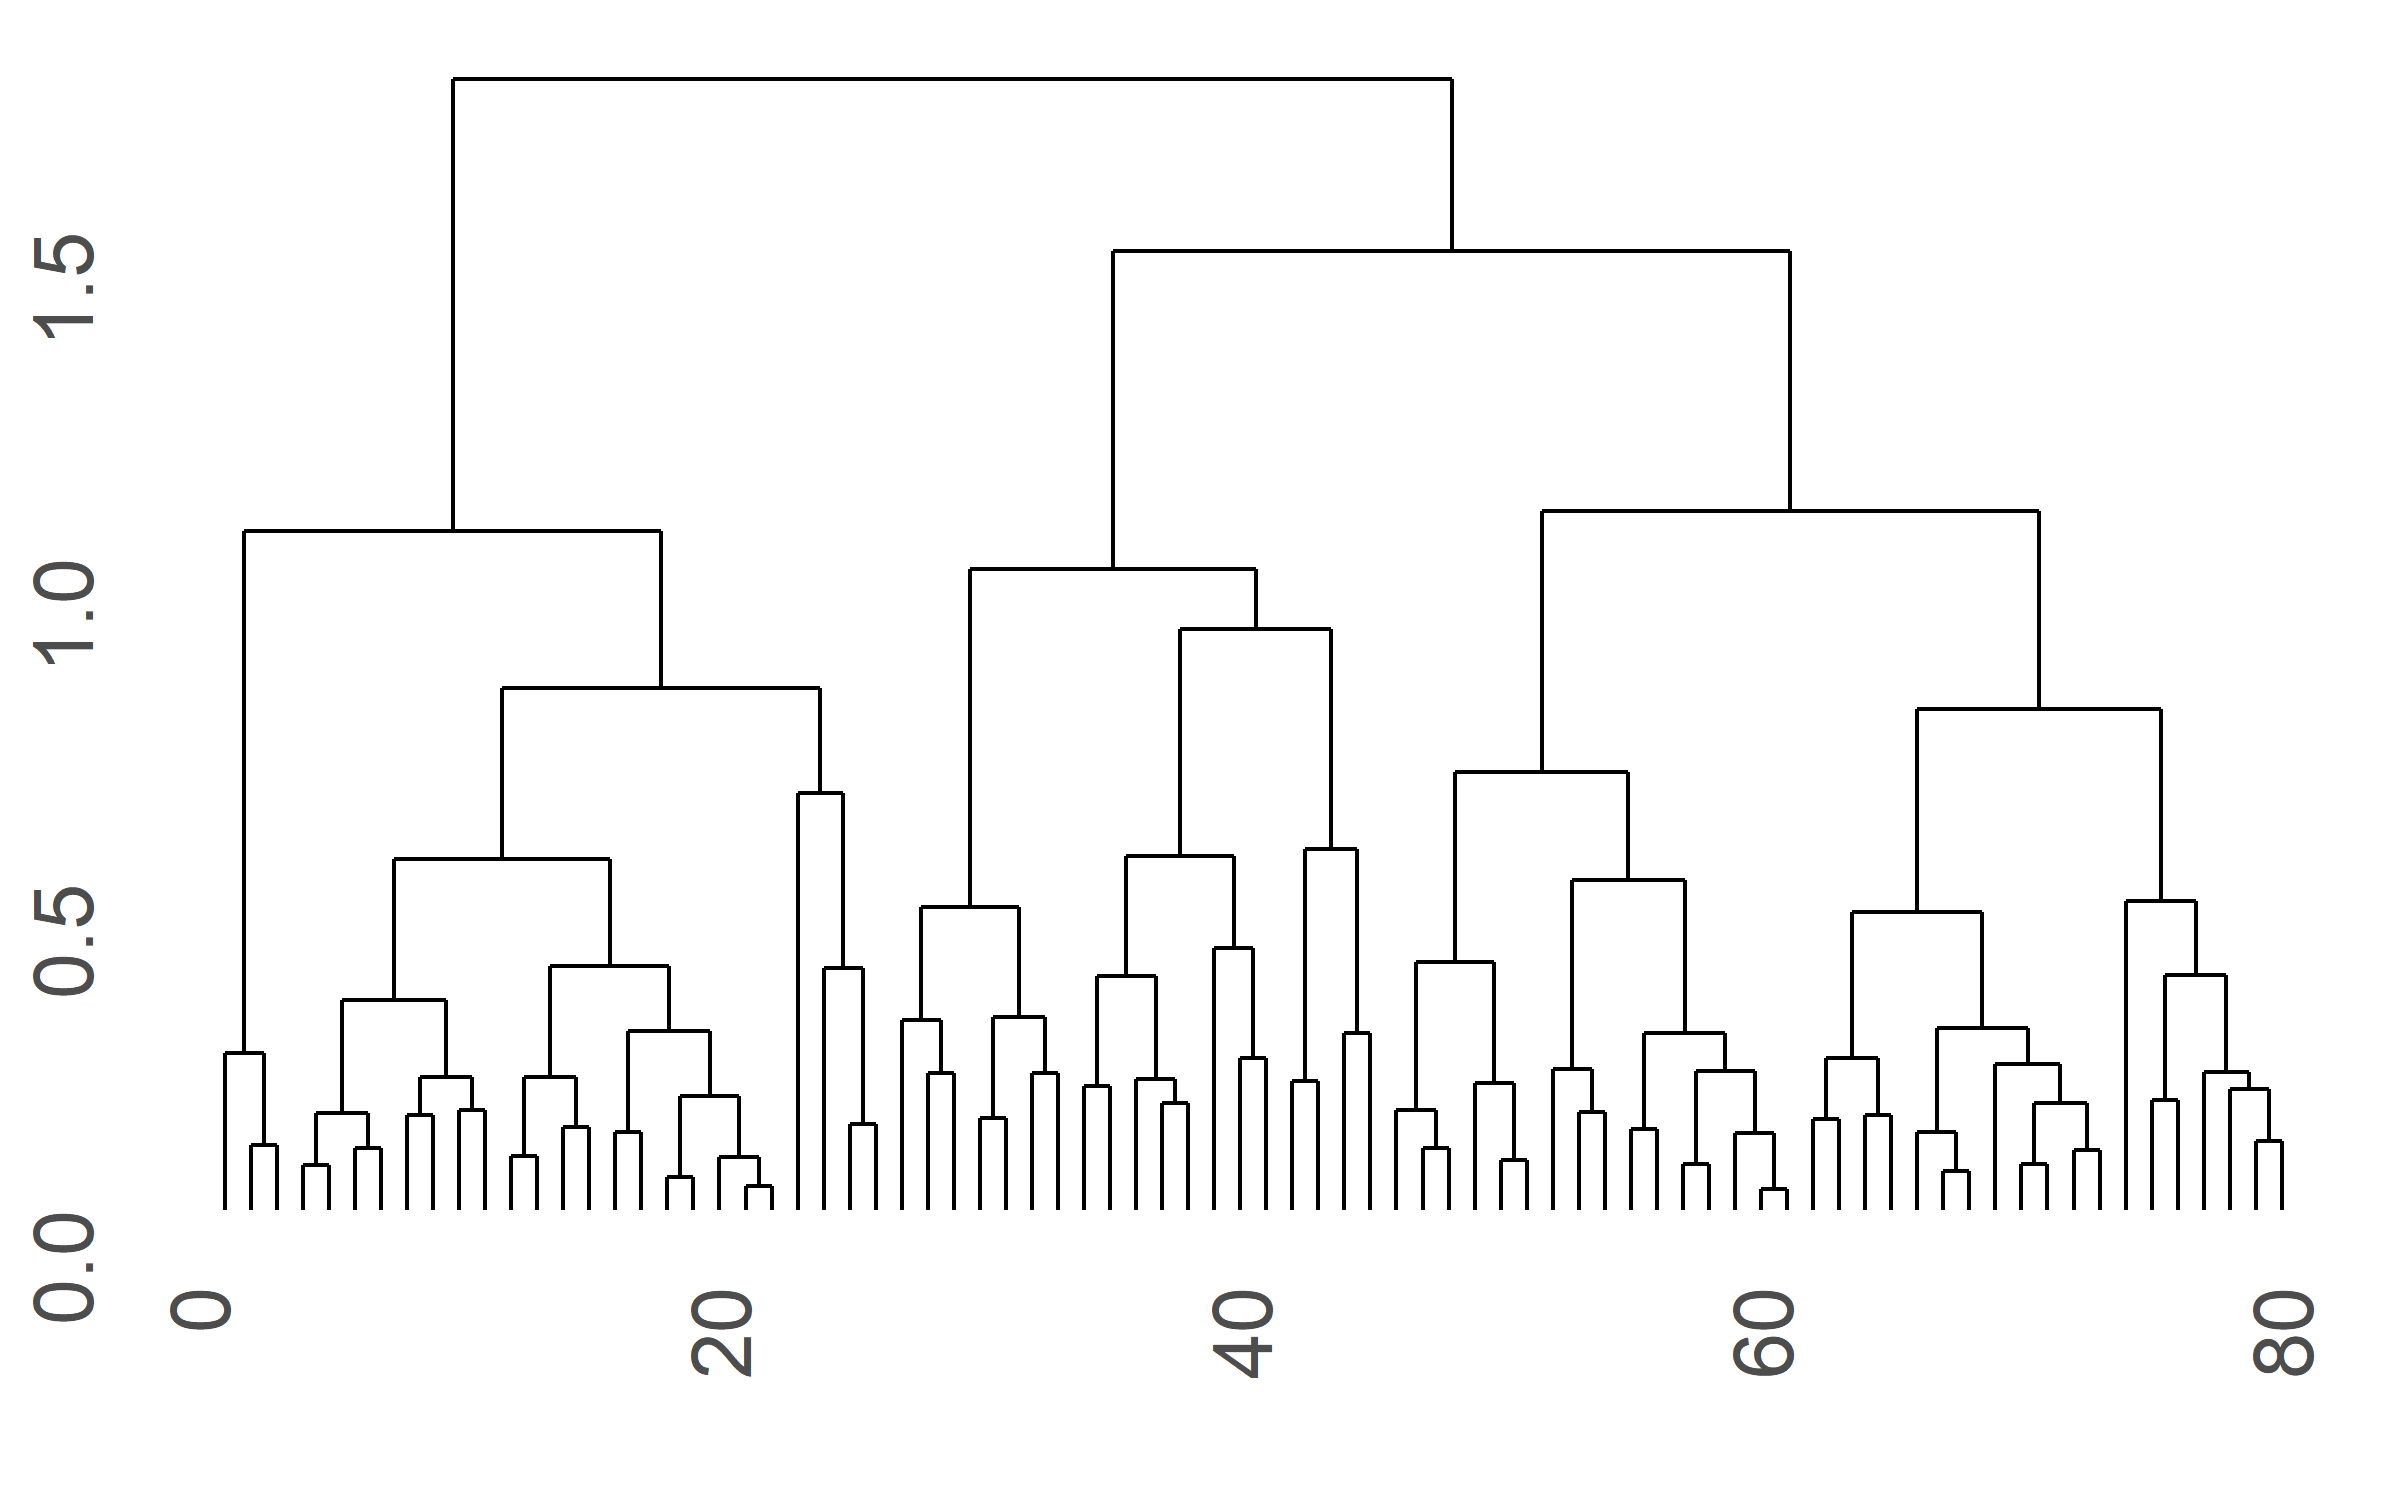
\includegraphics[width=0.8\textwidth]{img/dendrogram.png}
\caption{基频轮廓聚类树状图}
\label{den}
\end{figure}

将簇数设置为3时，得到聚类获得的基频轮廓如图\ref{f0}。

\begin{figure}[H]
\centering
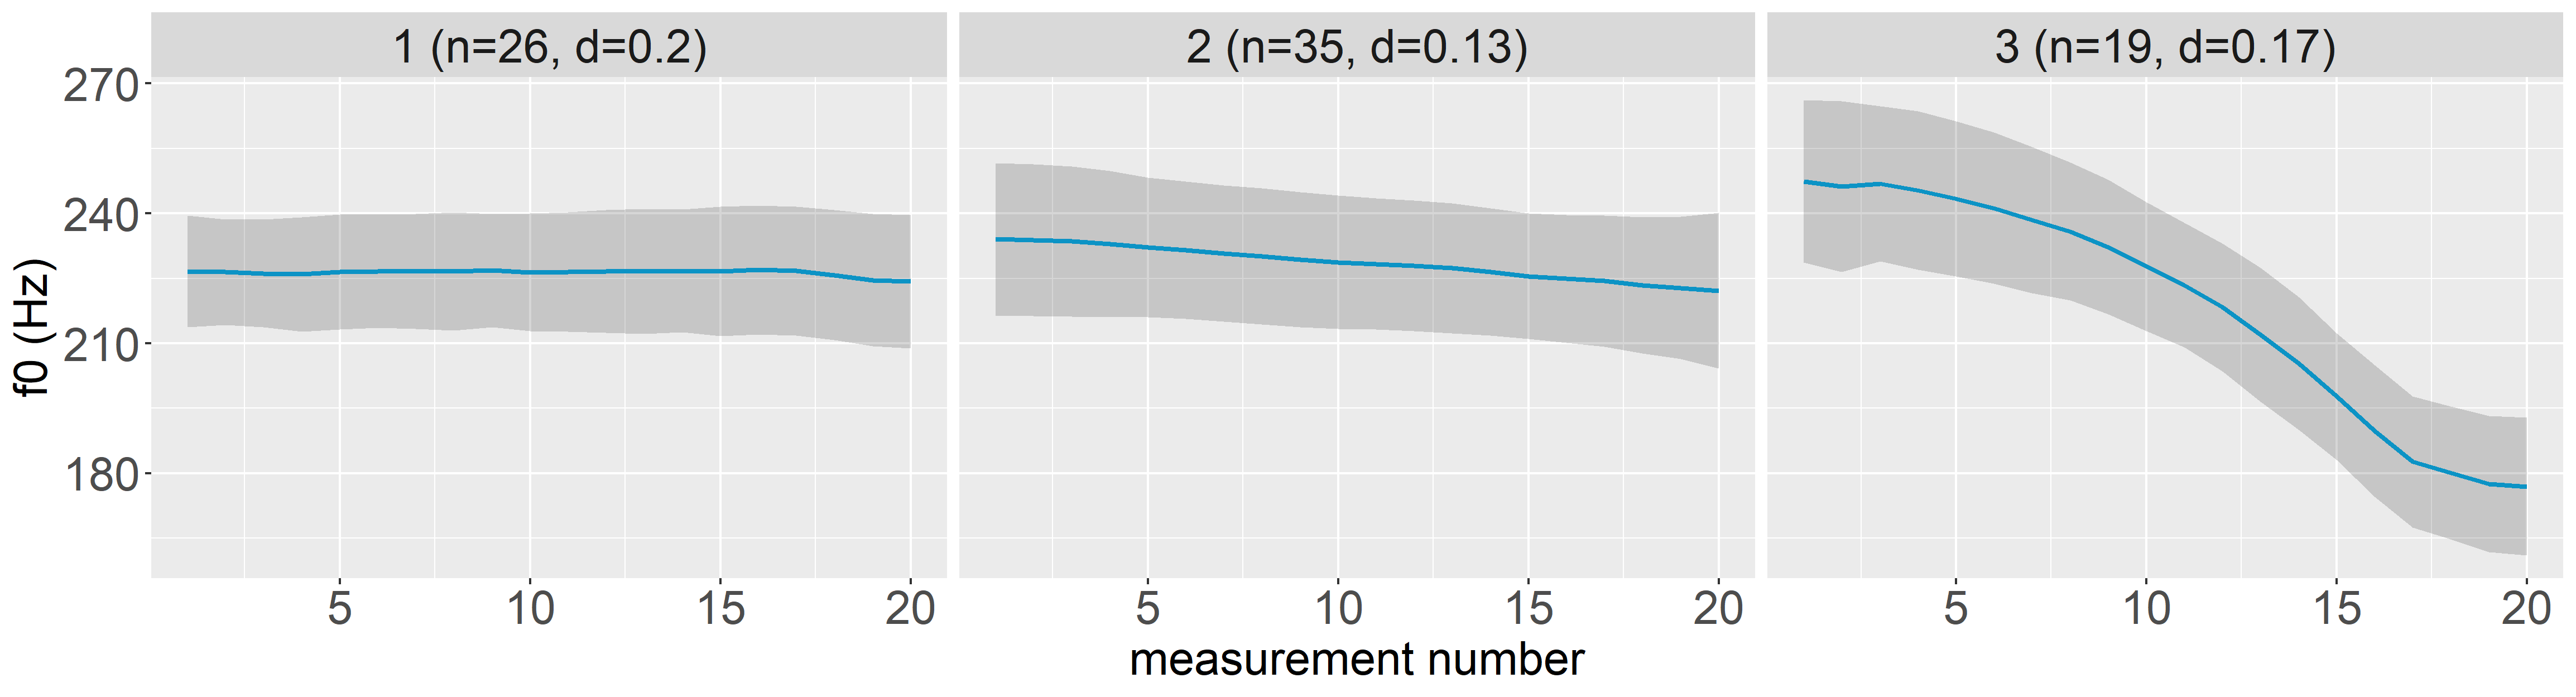
\includegraphics[width=0.8\textwidth]{img/plot_3.png}
\caption{基频轮廓}
\label{f0}
\end{figure}

其中簇1、2、3与人工标注的声调[H]、[HL]的对应如列联表\ref{toneclus}所示。

\begin{table}[H]
    \vspace{5pt}
    \centering
    \caption{声调-聚类簇列联表}
    \label{toneclus}
\begin{tabular}{c|ccc}
   \toprule
    \textit{} & 簇1 & 簇2 & 簇3 \\
    \midrule
  H & 25 & 25 & 0  \\
  HL & 1  & 10 & 19 \\
   \bottomrule
\end{tabular}
\end{table}

高调[H]样本主要集中于簇1和簇2，降调[HL]的样本集中在簇3，少部分分布在簇2。在“聚类结果与声调相互独立”的原假设下计算得到的期望频数与观测频数差异显著，$\chi ^{2}(2) = 45.42$，对应的显著性水平为$p = 1.37\times 10^{-10} \lll  0.001$。由此可见，聚类结果与声调之间存在高度相关性。

根据聚类结果和人工测量的基频，可以得出米亚罗话[H]调基频大约在210-240Hz之间，[HL]调基频大约从240-270Hz下降到150-180Hz。

以此为基准，可以测量出米亚罗话的表层声调在各个音节下有三种调型，如表\ref{to}所示。

\begin{table}[H]
    \vspace{5pt}
    \centering
    \caption{调型表}
    \label{to}
\begin{tabular}{c|cccc}
   \toprule
    & 单音节 & 双音节  & 三音节    & 四音节      \\
    \midrule
  (a) & H   & L.H  & L.H.H  & L.H.H.L  \\
(b) & HL  & L.HL & L.H.HL & L.H.H.HL \\
(c) & L   & H.L  & H.H.L  & L.H.H.L \\
   \bottomrule
\end{tabular}
\end{table}

其中，调型(c)仅仅应用在动词的屈折形态以及状貌词上。其他词汇均应用调型(a)和(b)。可以看出，米亚罗话每个词汇的表层声调似乎是可预测的，在下一节将具体讨论米亚罗话的底层声调和其如何推导到表层声调。

\section{底层声调}

正如\textcite{hsieh1999theoretical}和\textcite{lin2012no}所论证的，四土嘉绒语卓克基话的表层声调系统是可预测的。林幼菁指出卓克基话存在一个缺性声调（privative tone）系统，其底层是降调和零声调的对立，而在表层展现为词末音节降调和高低调的对立；且根据底层声调可以确定表层声调的表现。在米亚罗话中，底层同样存在词末音节降调和零声调的对立。本文采用V标示词末音节为零声调，V̂标示词末音节为降调。

米亚罗话的零声调和降调的对立具有词汇辨义作用，如表\ref{tonex}所示。

\begin{table}[H]
    \vspace{5pt}
    \centering
    \caption{双音节词汇声调最小对}
    \label{tonex}
\begin{tabular}{cc|cc}
   \toprule
    /$\varnothing$/ &  & /HL/ & \\
    {[L.H]} & & [L.HL] & \\
    \midrule
  {[kɐwu]} & “左面” &  [kɐ-wû] & “给” \\
   {[tə-mə]} & “女人” & [tə-mə̂] & “天空/雨” \\
   \bottomrule
\end{tabular}
\end{table}

米亚罗话零声调词应用调型(a)和(c)。生成零声调词需要应用的规则有：

\begin{enumerate}
    \setlength{\itemsep}{-0.3em}
    \item 音步分解（左）：从词的左端分解出双拍抑扬音步。
    \item 音步分解（右）：从词的右端分解出双拍扬抑音步。
    \item 弱化音步：余下的单音节均划为单拍音步。
    \item 强制高调：每个音步中心成分指派高调[H]。
    \item 插入高调：两个高调之间不带调值的音节指派高调[H]。
    \item 默认低调：剩余不带声调的音节指派低调[L]。
\end{enumerate}

相较于卓克基话的声调生成规则（\cite{lin2012no}），米亚罗话的的主要区别是弱化音步操作会对所有的单音节生效，而非卓克基话仅对非词首音节生效。

调型(a)的的规则使用顺序是：音步分解（左）、音步分解（右）、弱化音步、强制高调、插入高调、默认低调。如下例：

\begin{table}[H]
\begin{tabular}{ll}
           & kə-mə.rtsep “辣的” \\
词语         & kə.mə.rtsep      \\
1. 音步分解（左） & (kə.\textbf{mə})rtsep     \\
2. 音步分解（右） & N/A              \\
3. 弱化音步    & (kə.\textbf{mə})(\textbf{rtsep})   \\
4. 强制高调    & (kə.\ruby[g]{\textbf{mə}}{H})(\ruby[g]{\textbf{rtsep}}{H})   \\
5. 插入高调    & N/A              \\
6. 默认低调    & \ruby[g]{kə}{L}.\ruby[g]{mə}{H}.\ruby[g]{rtsep}{H}     \\
表面形式       & {[}L.H.H{]}     
\end{tabular}
\end{table}

调型(c)的规则使用顺序是：音步分解（右）、音步分解（左）、弱化音步、强制高调、插入高调、默认低调。如下例：

\begin{table}[H]
\begin{tabular}{lll}
           & ndze.ndzet “蹑手蹑脚” & te-wɐ.net “点灯（命令式）” \\
词语         & ndze.ndzet        & te.wɐ.net           \\
1. 音步分解（右） & (\textbf{ndze}.ndzet)        & te.(\textbf{wɐ}.net)           \\
2. 音步分解（左） & N/A               & N/A                 \\
3. 弱化音步    & N/A               & (\textbf{te})(\textbf{wɐ}.net)           \\
4. 强制高调    & (\ruby[g]{\textbf{ndze}}{H}.ndzet)        & (\ruby[g]{\textbf{te}}{H})(\ruby[g]{\textbf{wɐ}}{H}.net)           \\
5. 插入高调    & N/A               & N/A                 \\
6. 默认低调    & \ruby[g]{ndze}{H}.\ruby[g]{ndzet}{L}        & \ruby[g]{te}{H}.\ruby[g]{wɐ}{H}.\ruby[g]{net}{L}           \\
表面形式       & {[}H.L{]}         & {[}H.H.L{]}        
\end{tabular}
\end{table}

表面调型(b)只有词末音节会指派[HL]调，其余规则使用顺序与调型(a)相同。如下例：

\begin{table}[H]
\begin{tabular}{ll}
           & kʰa.jpɐ.lu.lu “蝴蝶” \\
词语         & kʰa.jpɐ.lu.lu      \\
1. 音步分解（左） & (kʰa.\textbf{jpɐ})lu.\ruby[g]{lu}{HL}      \\
2. 音步分解（右） & (kʰa.\textbf{jpɐ})(\textbf{lu}.\ruby[g]{lu}{HL})      \\
3. 弱化音步    & N/A                \\
4. 强制高调    & (kʰa.\ruby[g]{\textbf{jpɐ}}{H})(\ruby[g]{\textbf{lu}}{H}.\ruby[g]{lu}{HL})      \\
5. 插入高调    & N/A                \\
6. 默认低调    & \ruby[g]{kʰa}{L}.\ruby[g]{jpɐ}{H}.\ruby[g]{lu}{H}.\ruby[g]{lu}{HL}      \\
表面形式       & {[}L.H.H.HL{]}    
\end{tabular}
\end{table}